\section{Model of Motor and Wheel}
%An overall block diagram of the model of the motor and wheels can be seen on \autoref{fig:motorOverall}.
The model of the motors and wheels can be split into two parts; an electrical part and a mechanical part, since the two parts can be analyzed separately, though they are connected. This is due to the feedback that is present between the rotational velocity and the voltage, when modelling a motor \citep[15]{modelnote}.\\
The electrical model gives an output describing the motor current, $I_a(t)$. This is linked to the motor torque through the motor constant, $k_t$ \citep[p. 14]{modelnote}.\\
The mechanical part of the motor model describes both the motors, gears and wheels, since these are all connected. The mechanical part of the model has the angular velocity of the wheel, $\omega_w$ as output.
%A wheel model is also included to give the output of the motors and wheels model, that is the force applied, $F_F$, to the system by the motors and wheels.
A feedback is present in the system from $\omega_w$ to the applied voltage $v_a$, due to the back-EMF in the motor.\\
%\begin{figure}[H]
%\centering
%\scalebox{0.9}{
%\input{figures/overallMotor.rasmus}
%}
%\caption{An overall system diagram of the motor, gears and wheels.}
%\label{fig:motorOverall}
%\end{figure}
In the following, the electrical motor model is derived. Then, a mechanical model of the motors and wheels is put up. These two models can then be combined.\\
%\textbf{As the final step in the model of the motors and wheels, an expression for the applied force, $F_F$ is made, which can then be merged with the motor-wheel transfer function.}\\
Note that the modelling will be based on a single motor and wheel system, as the two motors and wheels on the segway are assumed identical. However, when deriving the expression for the applied force, $F_F$, both motors and wheels in the system are accounted for.
%After this, the inverted pendulum is modelled. This model can be combined with the motors and wheels model, to get the transfer function for the entire plant, as described in \autoref{fig:modelOverall}.\\
%In the following section, the electrical part of the motor is modelled.
\subsection{Electrical Motor Model}
The electrical part of a motor can be modelled using a resistor, $R_a$, an inductor, $L_a$, and a voltage generator, $V_e$, which delivers a voltage proportional to the motor's angular velocity $\omega_m$, also known as the back-EMF voltage \citep[p. 15]{modelnote}. This can be seen in \autoref{fig:motor_electrical}, where the input voltage, $V_a$, and the motor current, $I_a$, are shown, with the index $a$ denoting the armature of the motor. This model assumes that it is a permanent magnet DC motor that is used \citep[p. 15]{modelnote}, but as explained in section \ref{subsec:motors}, the motors used are of this type, meaning the model structure is valid.
\begin{figure}[H]
\centering
\begin{circuitikz}[american voltages]

	% electrical equivalent circuit
	\draw (0,0) to[V, v^=$V_a$] (0,3);
	\draw (0,3) to[R, i>^=$I_a$, l=$R_a$] (3,3);
	\draw (3,3) to[L, l=$L_a$] (4,3);

	\draw (4,3) -- (5,3);
	\draw (5,0) to[V, v_=\mbox{$V_e = k_e\omega_m$}] (5,3);
	\draw (0,0) -- (5,0);

\end{circuitikz}
\caption{Electrical curcuit equivalent of a DC motor.}
\label{fig:motor_electrical}
\end{figure}
Kirchoff's voltage law is applied to the circuit yielding the following expression:
\begin{equation}
0 = V_a(t) - R_a\cdot I_a(t) - L_a \dot{I_a}(t) - V_e(t) \label{eq:kirchoffsV}
\end{equation} 
\begin{where}
\va{$V_a(t)$}{is the motor input voltage}{V}
\va{$R_a$}{is the motor resistance}{$\Omega$}
\va{$L_a$}{is motor inductance}{H}
\va{$I_a(t)$}{is motor current}{A}
\va{$V_e(t)$}{is the back-EMF}{V}
\end{where}

%The equation is Laplace transformed to give the following:
%\begin{equation}
%\label{eq:electricMotor}
%0 = V_a(s) - R_a\cdot I_a(s) - s L_a I_a(s) - V_e(s)
%\end{equaeetion}

%$V_e$ is proportional to the motor velocity \citep[p. 15]{modelnote}, i.e.:
\clearpage
The back-EMF is directly proportional to the rotational speed of the motor:
\begin{equation}
V_e(t) = k_e \cdot\omega_m(t)
\end{equation}
\begin{where}
\va{$\omega_m(t)$}{is the rotational speed of the motor}{$\text{rad}/$s}
\va{$k_e$}{is the back-EMF constant}{V$/{\frac{\text{rad}}{s}}$}
\end{where}

Now, the expression for $V_e(t)$ can be inserted in \autoref{eq:kirchoffsV}. The equation is isolated for $I_a(t)$, since the current is the interface between the electrical and mechanical parts of the model. It is assumed that $\dot I_a(t) = 0$, since the electrical time constant is usually much higher than mechanical time constant \citep[p. 74]{sou:Feedback}. This yields \autoref{eq:electricMotor2}.
\begin{equation}
\label{eq:electricMotor2}
I_a(t) = \frac{1}{R_a} \left( V_a(t) - k_e \cdot \omega_m(t) \right)
\end{equation}
The torque of a motor is proportional to the current \citep[p. 14]{modelnote}:
\begin{equation}
\tau_m(t) = k_t \cdot I_a(t)
\label{eq:currenttau11}
\end{equation}
\begin{where}
\va{$\tau_m(t)$}{is the torque of the motor}{Nm}\\
\va{$k_t$}{is the motor constant}{Nm/A}\\
\end{where}

Inserting the expression for the current $I_a(t)$ from \autoref{eq:electricMotor2} into \autoref{eq:currenttau11} gives the following:
\begin{equation}
\label{eq:voltageToTorque}
\tau_m(t) = \frac{k_t}{R_a} \left( V_a(t) - k_e \omega_m(t) \right)
\end{equation}
%
%A block diagram of \autoref{eq:voltageToTorque} can be put up, see \autoref{fig:motorGearBlock}. Here, the input is the applied voltage $V_a(t)$, and the output the motor angular velocity, $\omega_m(t)$.
%
%Notice that a block describing the mechanical motor-wheel system has been inserted to transfer from torque, $t_m(t)$ to the angular velocity of the motor, $\omega_m(t)$. 
%%A gear transfer function is also inserted, to obtain the angular velocity of the wheel, $\omega_w(s)$ from the motor angular velocity, $\omega_m(s)$.
%
%\begin{figure}[H]
%\centering
%\input{figures/electricalMotor.rasmus}
%\caption{A block diagram of the motor and gearing.}
%\label{fig:motorGearBlock}
%\end{figure}

A model for the gears and wheel needs to be determined to find the torque $\tau_a$ that is applied to the segway, since the inertias and dampers in the gear-wheel setup influences this. This is done in the following section.
%In the next section, the transfer function for the mechanical system and the gears, describing the relationship between motor torque $\tau_m(s)$ and the rotational speed of the motor, $\omega_m(s)$, as well as the relationship between $\omega_m(s)$ and $\omega_w(s)$.

%In the feedback on \autoref{fig:motorGearBlock}, a transfer function describing the gearing is also needed, to describe the motor angular velocity $\omega_m(s)$ based on the wheel angular velocity, $\omega_w(s)$. These two gear transfer functions are derived in the following section. 
%To transfer from $\omega_w$ to $\omega_m$, the inverted gear ratio is inserted, since this is the connection between the two angular velocities.

%Ideally, the function in \autoref{eq:voltageToTorque} is turned into a transfer function describing the relationship between input voltage and motor torque. This is however not possible, since the gearing transfer functions are not yet known. Thus, these need to be determined before the transfer function for the system can be put up. 
%In the next section, the transfer function for the gears, describing the relationship between motor torque $\tau_m(s)$ and the rotational speed of the outer wheel, $\omega_w(s)$ can found. 
\subsection{Mechanical Motor and Wheel Model}
%The transfer function from motor torque $\tau_m$, to the angular velocity of the motor, $\omega_m$, is now to be found.
A model for the mechanical behaviour of the motors and wheels is to be found, so it can be combined with the electrical model for the motors, thus forming the combined model for the motors and wheels. \\
It is necessary to take the entire mechanical system, eg. both wheels and gearing ratios, into account, as these affect the motor's rotation.

\subsubsection{Gear relations}
First, the configuration of the gears are determined before the modelling can begin. The motor and wheel system consists of a DC motor, which has a gear mounted. The output of this gear is applied to the motor shaft, onto which a secondary gear is mounted. The inner wheel gear is mounted directly on the shaft, and thus has the same angular velocity as the motor. Therefore their inertia can be seen as one, being the shaft inertia. The configuration of the gears can be seen in \autoref{fig:gears}.
\begin{figure}[H]
\centering
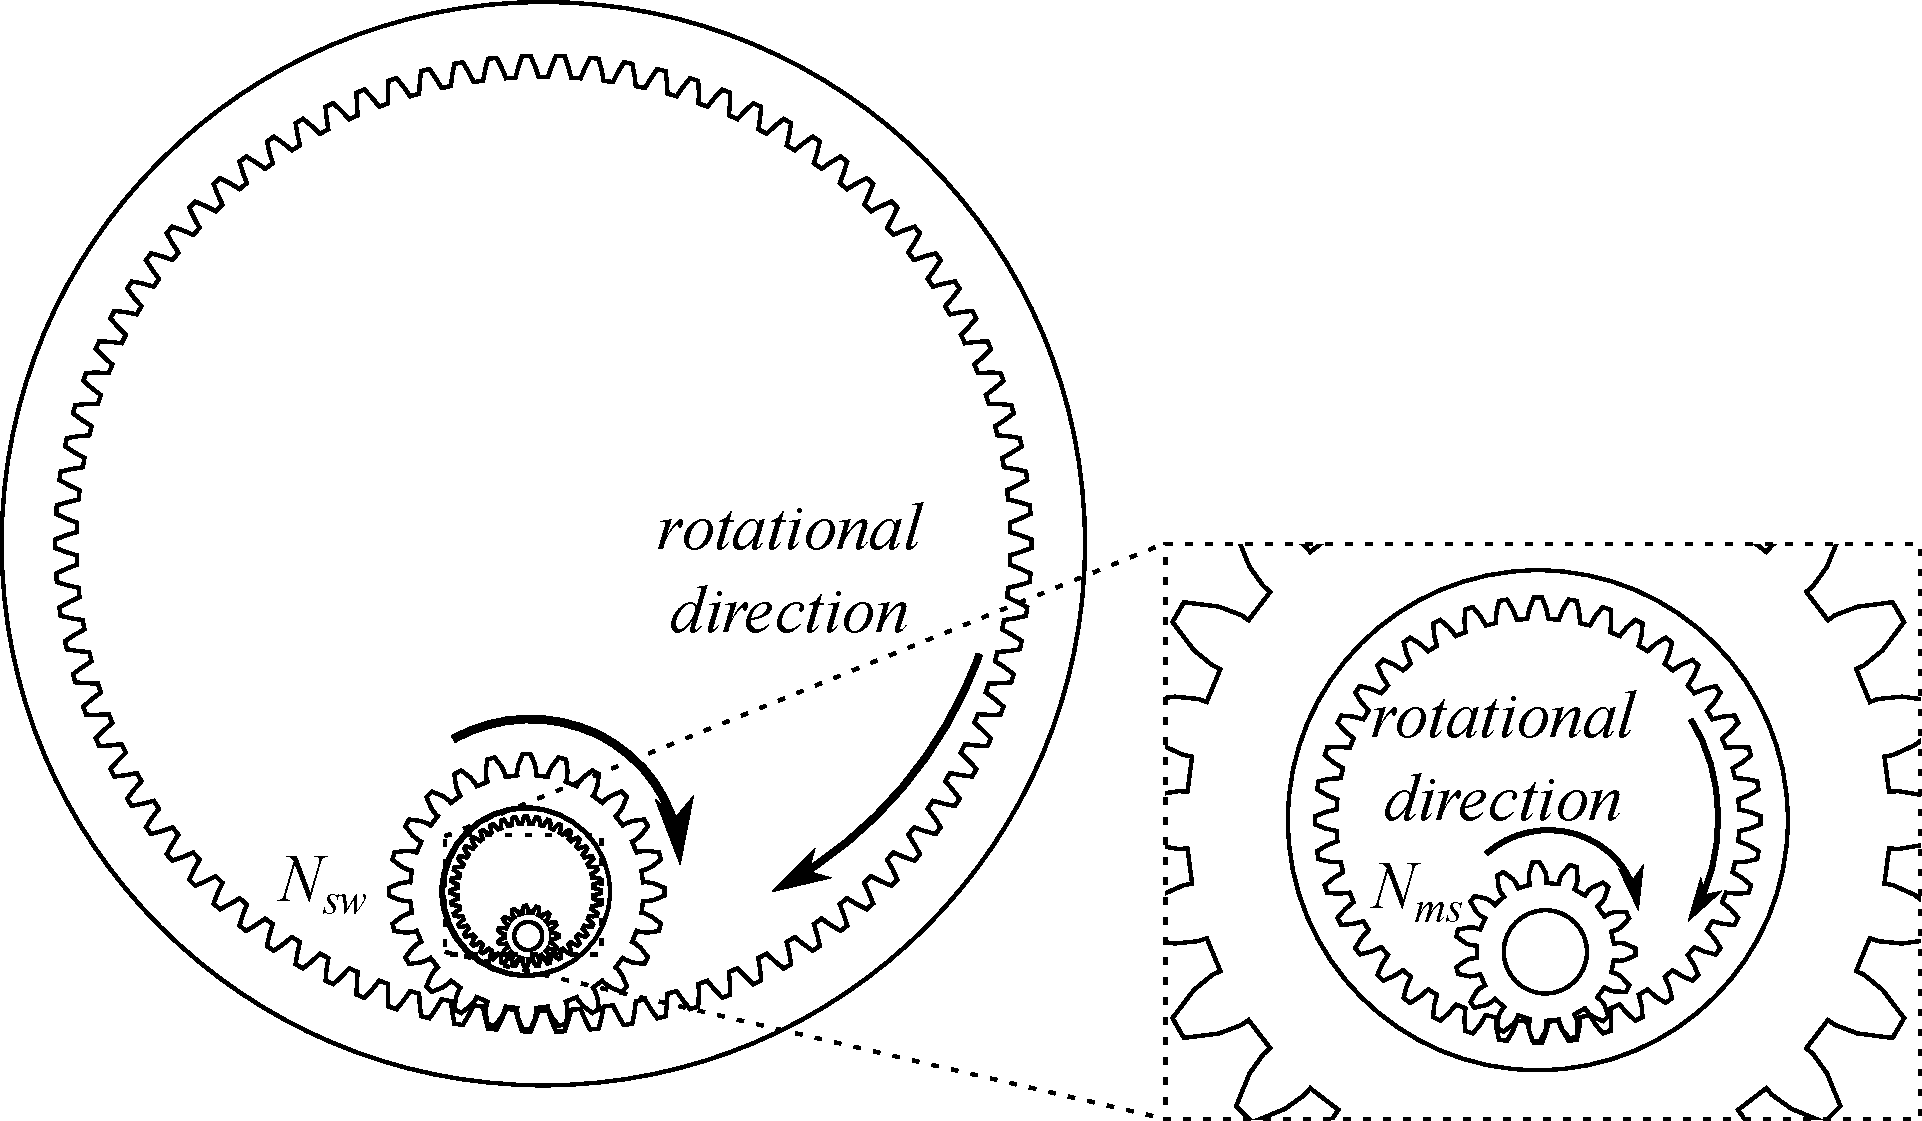
\includegraphics[width=0.75\textwidth]{figures/gears.pdf}
\caption{The different parts of the wheel's rotational system and its relative direction of rotation along with the gear ratios, $N_{ms}$ and $N_{sw}$.}
\label{fig:gears}
\end{figure}
In \autoref{fig:gears} the gear ratio between the motor and shaft is shown as $N_{ms}$, and the gear ratio for the shaft and wheel as $N_{sw}$.
\begin{figure}[H]
\centering
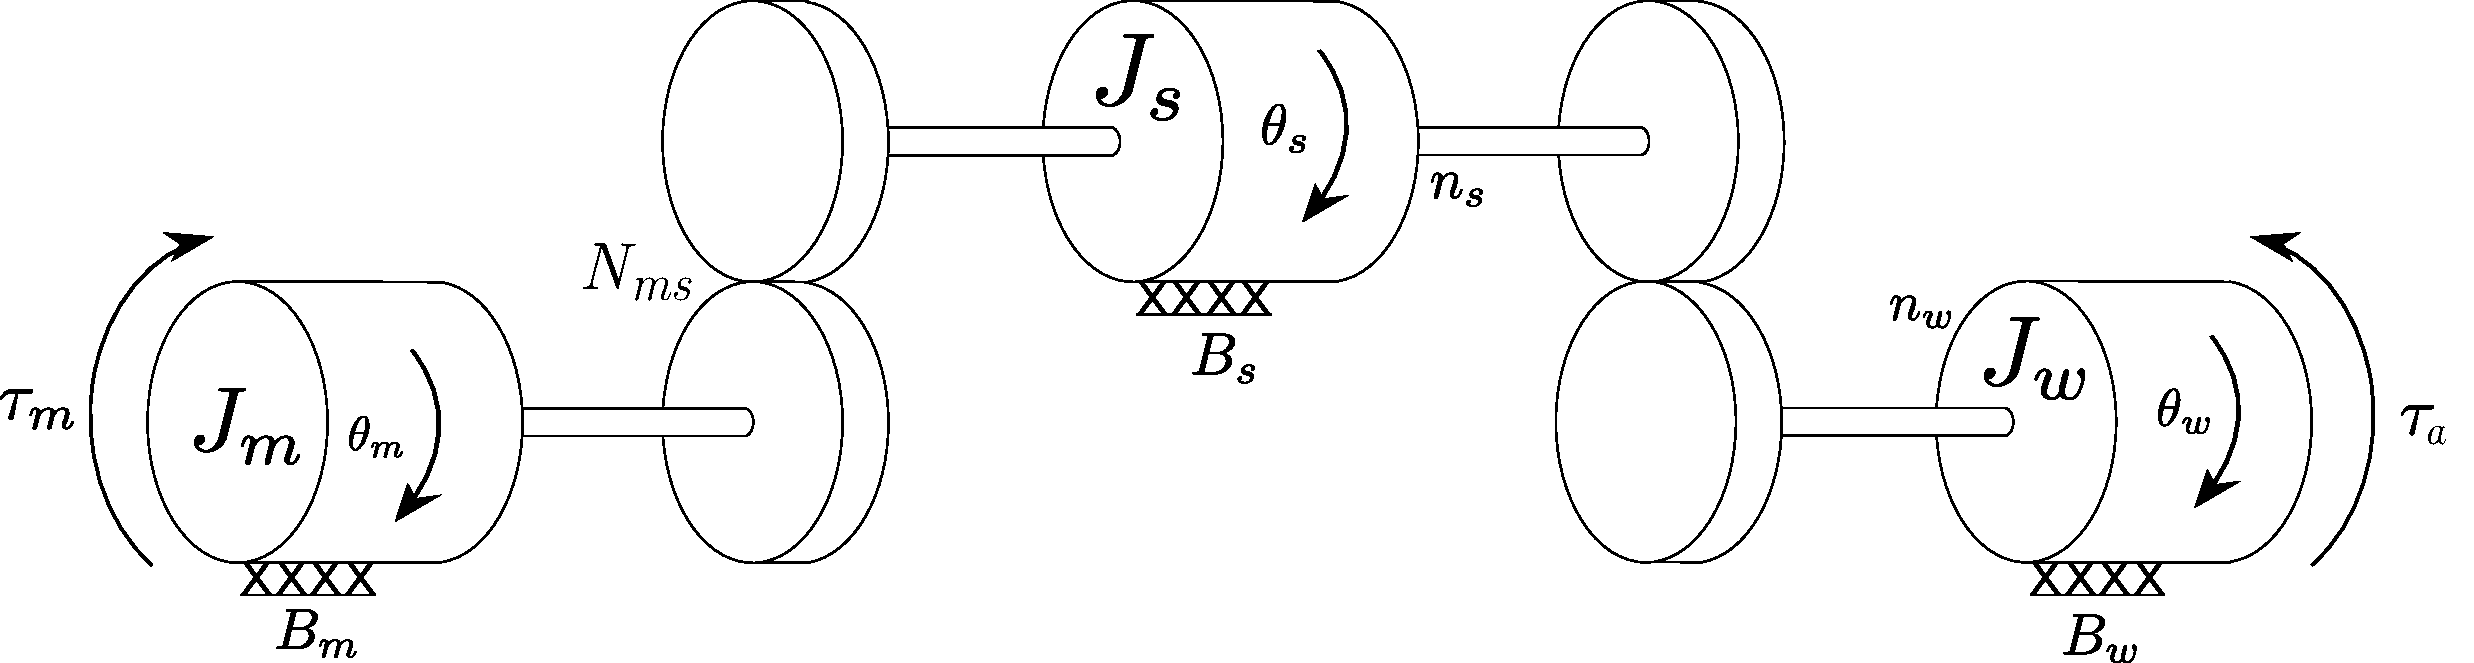
\includegraphics[width=\textwidth]{figures/motorRotationalDiagram.pdf}
\caption{Mechanical model of the motor and wheel setup.}
\label{fig:motorRotational}
\end{figure}

The gear ratio is used to determine the relation between angle and its derivatives for two or more rotational objects. The basis for determining is \autoref{fig:gearsRelation}, where it is assumed that there is no sliding between two gears. A torque $\tau_1$ is applied to the inner gear, giving it a certain angular position, $\theta_1$. The second gear also has a torque, $\tau_2$ and an angular position, $\tau_2$. Since the two gears have to move the same amount when rotating, as no slipping is assumed, \autoref{eq:gearRatio} can be put up, from which the gear ratio can be determined.

\begin{figure}[H]
\centering
\scalebox{1}{\input{figures/MotorAndWheel.ralf}}
\caption{Correlation of gears.}
\label{fig:gearsRelation}
\end{figure}

\begin{equation}
\theta_1r_1 = \theta_2r_2 \Rightarrow N = \frac{r_1}{r_2} = \frac{\theta_2}{\theta_1} = \frac{\omega_2}{\omega_1}
\label{eq:gearRatio}
\end{equation}
\begin{where}
\va{$N$}{The gear ratio}{1}
\va{$\theta_1$}{Angle of the inner gear}{rad}
\va{$\theta_2$}{Angle of the outer gear}{rad}
\va{$r_1$}{The radius of the inner gear}{m}
\va{$r_2$}{The radius of the outer gear}{m}
\va{$\omega_1$}{Angle velocity of the inner gear}{rad/s}
\va{$\omega_2$}{Angle velocity of the outer gear}{rad/s}
\end{where}

This, however, does not yield the relation between the torque of the gears and the gear ratio. This relation can be obtained through steady state analysis of each gear. This yields \autoref{eq:steadyGear1} and \autoref{eq:steadyGear2} for the inner and outer gear respectively, since the force of the two gears are of the same magnitude, i.e. $F_{g1}$ = $F_{g2}$ = $F_g$. This is because the force one gear excerts on the other is balanced by an equal, but opposite force, in correlation with Newton's 3rd law of motion. Based on this, it is possible to put up the following equations:
\begin{align}
\tau_1 - r_1\cdot F_g = 0 \label{eq:steadyGear1}
\\
\tau_2 - r_2\cdot F_g = 0\label{eq:steadyGear2}
\end{align}
\begin{where}
\va{$F_g$}{Translatoric force that works against the gear.}{N}
\end{where}

Thus, the gear ratio affects the relation between the torque in the two gears as shown in \autoref{eq:torqueRelation}.
\begin{equation}
\frac{\tau_1}{\tau_2} = \frac{r_1}{r_2} = N
\label{eq:torqueRelation}
\end{equation}

To describe the relation of the torque and the angle for two or more gears, the gear ratio, N, must be determined. This is done through the number of cogs in each cogwheel, as this can be thought of being equivalent to the wheel radii, which has previously been used to determine the gear ratio. From \autoref{subsec:wheels}, it's known that $n_s = 25$ and $n_w = 90$. From these, the gear ratio can be found.

\begin{equation}	
N_{sw} = \frac{n_s}{n_w} = \frac{\theta_w(t)}{\theta_s(t)} = \frac{25}{90} \approx 0.2778
\label{Nsw}
\end{equation}
\begin{where}
\va{$N_{sw}$}{is the shaft-wheel gear ratio}{1}\\
\va{$n_s$}{is number of cogs on the motor gear}{1}\\
\va{$n_w$}{is number of cogs on the wheel}{1}\\
\va{$\theta_s(t)$}{is the motor angle}{rad}\\
\va{$\theta_w(t)$}{is the wheel angle}{rad}\\
\end{where}

From \citep{gear} the gear ratio from motor to shaft is known:
\begin{equation}
N_{ms} = \frac{1}{19} \approx 0.053
\label{Nms}
\end{equation}
With the gear relations determined, it is now possible to derive the mechanical motor and wheel model.
\vspace{0.4 cm}
\subsubsection{Derivation of Mechanical Motor and Wheel Model}
\vspace{0.3 cm}
Now that the configuration of the rotational system is known, the motor, shaft and wheel system can be drawn using ideal elements, i.e. inertias and dampers, which can be seen in \autoref{fig:motorRotational}. Note, that all gears are assumed to have an inertia and a friction as no gears are assumed ideal. Also note that the friction in the gears is modelled as a damper, and thus each of the friction torques can be described in the same way as the friction torque for the shaft shown here: $\tau_{B_s}(t) = B_s \cdot \omega_s(t)$. The coulomb friction which is also present is not taken into account, due to the fact that an offset in the software can take care of this non-linearity, which is not easily modelled.\\
\clearpage
In \autoref{fig:motorRotational} it is seen how the motor connects to the shaft, which again connects to the wheel. All connections are made through gears. The constants $n_s$ and $n_w$, are the number of cogs on the shaft and wheel cog-wheels. These are used to determine the gear ratios.\newpar
The input torque to the motor $\tau_m(t)$, see \autoref{fig:motorRotational}, sets the direction of all the resultant angular positions, and therefore also angular velocities and angular accelerations in accordance with \autoref{fig:gears}.\\
The free body diagrams of the motor, shaft and wheel are illustrated in \autoref{fig:FBDMotorShaftWheel}. %In the motor part \autoref{fig:FBDMotor}, the motor torque, $\tau_m$, is inserted along with a friction torque, $\tau_{B_m}$, and a gearing torque transferring torque to the wheel.
%In the wheel part \autoref{fig:FBDWheel}, the gear torque, $\tau_{G_w}$, is inserted, along with a friction torque. The resultant torques are also shown.
\begin{figure}[H]
\centering
\begin{subfigure}[b]{0.3\textwidth}		
        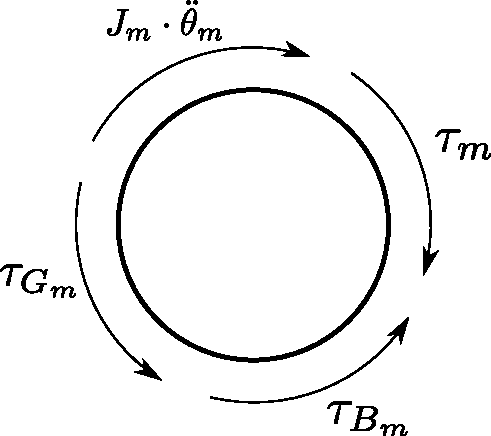
\includegraphics[width=0.98\textwidth]{figures/FBD/FBDMotor.pdf}
        \vspace{3.5mm}
        \caption{FBD of rotational system for the motor.}
        \label{fig:FBDMotor}
    \end{subfigure} 
    \hspace{4mm} 
\begin{subfigure}[b]{0.3\textwidth}
        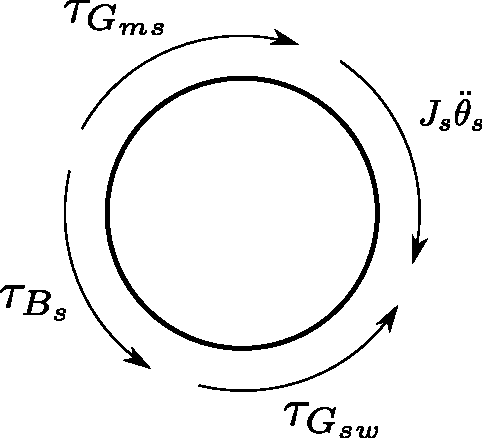
\includegraphics[width=0.95\textwidth]{figures/FBD/FBDShaft.pdf}
        \vspace{2mm}
        \caption{FBD of rotational system for the shaft.}
        \label{fig:FBDshaft}
    \end{subfigure}  
    \hspace{4mm} 
\begin{subfigure}[b]{0.3\textwidth}
        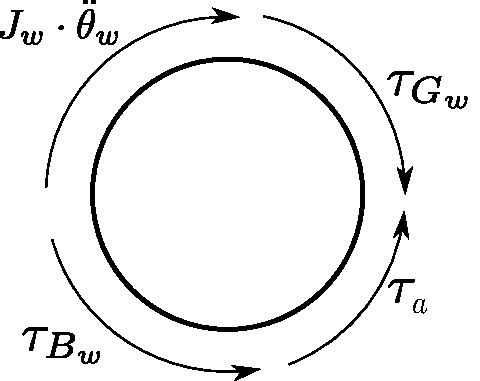
\includegraphics[width=0.95\textwidth]{figures/FBD/FBDWheel.pdf}
        \vspace{5mm}
        \caption{FBD of rotational system for the wheel.}
        \label{fig:FBDWheel}
    \end{subfigure}
\caption{Free body diagrams of the three rotational systems.}
\label{fig:FBDMotorShaftWheel}
\end{figure}
Note that the following relationships between the gear torques exist, based on the gear ratios: 
\begin{equation}
\tau_{G_{ms}}(t) = \tau_{G_m}(t) \cdot \frac{1}{N_{ms}}
\label{gearTorqueMotor}
\end{equation}
\begin{equation}
\tau_{G_w}(t) = \tau_{G_{sw}}(t) \cdot \frac{1}{N_{sw}}
\label{gearTorqueWheel}
\end{equation}
\begin{where}
\va{$\tau_{G_{ms}}(t)$}{is the torque from motor to shaft}{Nm}\\
\va{$\tau_{G_m}(t)$}{is the torque to shaft from motor}{Nm}\\
\va{$\tau_{G_w}(t)$}{is the torque from shaft to wheel}{Nm}\\
\va{$\tau_{G_{sw}}(t)$}{is the torque to wheel from shaft}{Nm}\\
\end{where}

From \autoref{fig:FBDMotorShaftWheel}, the following differential equations can be put up:
\begin{align}
J_m\ddot\theta_m(t) &= \tau_m(t) -\tau_{G_m}(t) - \tau_{B_m}(t)\label{eq:DE1}\\
J_s\ddot\theta_s(t) &= \tau_{G_{ms}}(t) - \tau_{G_{sw}}(t) - \tau_{B_s}(t)\label{eq:DE2}\\
J_w\ddot\theta_w(t) &= \tau_{G_{w}}(t) - \tau_{B_w}(t) -\tau_a(t) \label{eq:DE3}
\end{align}

\begin{where}
\va{$J_m$}{is the motor moment of inertia}{$\text{kg} \cdot \text{m}^2$}\\
\va{$J_s$}{is the shaft moment of inertia}{$\text{kg} \cdot \text{m}^2$}
\va{$J_w$}{is the wheel moment of inertia}{$\text{kg} \cdot \text{m}^2$}
\va{$\ddot\theta_m(t)$}{is the angular acceleration of the motor}{$\text{rad}/\text{s}^2$}\\
\va{$\ddot\theta_s(t)$}{is the angular acceleration of the shaft}{$\text{rad}/\text{s}^2$}\\
\va{$\ddot\theta_w(t)$}{is the angular acceleration of the wheel}{$\text{rad}/\text{s}^2$}\\
\va{$\tau_m(t)$}{is the delivered torque from the motor}{$\text{rad}/\text{s}^2$}\\
\va{$\tau_{B_m}(t)$}{is the motor friction torque}{Nm}\\
\va{$\tau_{B_s}(t)$}{is the shaft friction torque}{Nm}\\
\va{$\tau_{B_w}(t)$}{is the wheel friction torque}{Nm}\\
\va{$\tau_{a}(t)$}{is the torque applied to the cart}{Nm}\\
\end{where}

In the following, a model for the motors and wheels system is obtained. This is done using the differential equations derived from the free body diagrams, see \autoref{eq:DE1}, \autoref{eq:DE2} and \autoref{eq:DE3}.
%\textbf{In the following, a transfer function for the gearing/wheel system is obtained. The input to the system is the motor torque, $\tau_m(t)$, and the output is the angular velocity of the wheel, $\omega_w(t)$.
%This is done using the differential equations derived from the free body diagrams, see \autoref{eq:DE1}, \autoref{eq:DE2} and \autoref{eq:DE3}. It is desired to combine these equations, to obtain a transfer function for the entire mechanical model.\todo{not looking for a transferfunction. Rewrite}}
\\The model is derived by working from the outside and in, starting with the equations for the wheel and inserting them to get an expression for the motor that includes the wheel and shaft.\\
The differential equation for the wheel rotational system, \autoref{eq:DE3}, states:
\begin{equation}
J_w\ddot\theta_w(t) = \tau_{G_{w}}(t) - \tau_{B_w}(t) - \tau_a(t) \nonumber
\end{equation}
The linear approximation of the friction torque, which is modelled as a damper, can be described as $\tau_{B_s}(t) = B_s \cdot \dot\theta_s(t)$. Inserting this together with the expression for the gear torque from \autoref{gearTorqueWheel} gives:
\begin{equation}
J_w \ddot\theta_s(t) N_{sw} = \tau_{G_{sw}}(t)\cdot \frac{1}{N_{sw}} - {B_{w}} N_{sw} \cdot \dot\theta_{s}(t) -\tau_{a}(t)
\end{equation}
%Laplace transforming the equation and isolating for $\tau_{G_{sw}}$ gives:
%\begin{equation}
%s^2 J_w N_{sw} \theta_s(s) = \tau_{G_{sw}}(s)\cdot \frac{1}{N_{sw}} - s {B_{w}} N_{sw} \cdot \theta_{s}(s)
%\end{equation}
%\begin{equation}
%\tau_{G_{sw}}(s) = \theta_s(s) \cdot N_{sw}^2 (s^2 J_w + s B_w) 
%\label{tauGSW}
%\end{equation}
Isolating for $\tau_{G_{sw}}$ gives:
\begin{equation}
\tau_{G_{sw}}(t) = J_w \ddot\theta_s(t) N_{sw}^2 + B_wN_{sw}^2\dot\theta_s(t) + \tau_a(t) \cdot N_{sw}
\label{tauGSW}
\end{equation}
Now that an expression for $\tau_{G_{sw}}(t)$ is obtained, it can be combined with the differential equation for the second rotational system, \autoref{eq:DE3}, which states:
\begin{equation}
J_s\ddot\theta_s(t) = \tau_{G_{ms}}(t) - \tau_{G_{sw}}(t) - \tau_{B_s}(t) \nonumber
\end{equation}
The friction can, as previously mention be described as $\tau_{B_s}(t) = B_s \cdot \dot\theta_s(t)$. Inserting this and isolating for $\tau_{G_{ms}}(t)$ yields:
\begin{equation}
\tau_{G_{ms}}(t) = \tau_{G_{sw}}(t) + B_s \cdot \dot\theta_s(t) + J_s\ddot\theta_s(t) 
\label{tauGSAlmost}
\end{equation}
\autoref{tauGSW} is inserted in \autoref{tauGSAlmost} together with the expression for the motor-shaft gear from \autoref{gearTorqueMotor}. An expression for $\tau_{G_m}(t)$ can thus be found:
%\begin{equation}
%\tau_{G_{ms}}(t) = \left(J_w \ddot\theta_s(t) N_{sw}^2 + B_wN_{sw}^2\dot\theta_s(t) + \tau_a(t)\right) + B_s \cdot \dot\theta_s(t) + J_s\ddot\theta_s(t) 
%\label{tauGS}
%\end{equation}
%Inserting the motor-shaft gear ratio, an expression for $\tau_{G_m}(t)$ can be obtained:
%\begin{equation}
%\tau_{G_{m}}(s)\frac{1}{N_{ms}} = \theta_m(s){N_{ms}}(s^2(J_s + N_{sw}^2 J_w) + s (B_s + N_{sw}^2 B_w))\label{tauGMAlmost}
%\end{equation}
\begin{equation}
\tau_{G_{m}}(t) = J_w \ddot\theta_m(t) N_{ms}^2 N_{sw}^2 + B_w N_{ms}^2 N_{sw}^2\dot\theta_m(t) + \tau_a(t)\cdot N_{ms} N_{sw} + B_s N_{ms}^2 \cdot \dot\theta_m(t) + J_s N_{ms}^2 \ddot\theta_m(t) 
\label{tauGM}
\end{equation}

This expression can be combined with the differential equation for the motor rotational system, as seen in \autoref{eq:DE1} and stated here:
\begin{equation}
J_m\ddot\theta_m(t) = \tau_m(t) -\tau_{G_m}(t) - \tau_{B_m}(t) \nonumber
\end{equation}
Inserting the expression for the friction torque, $\tau_{B_m}(t) = B_m \cdot \dot\theta_m(t)$ and $\tau_{G_{m}}(t)$ as found in \autoref{tauGM} yields \autoref{eq:tauM(t)} where the motor torque $\tau_m(s)$ has also been isolated:\vspace{0.3 cm}
%\begin{equation}
%s^2 J_m \theta_m(s) = \tau_m(s) - \tau_{G_{m}}(s) - s{B_m}\theta_m(s)
%\end{equation}
%
%The motor torque, $\tau_m(s)$ is isolated:
\begin{align}
\begin{split}
\tau_m(t) = &J_m\ddot\theta_m(t) + B_m \cdot \dot\theta_m(t)+ ( J_w \ddot\theta_m(t) N_{ms}^2 N_{sw}^2 + \\ & B_w N_{ms}^2 N_{sw}^2\dot\theta_m(t) + \tau_a(t)\cdot N_{ms} N_{sw} + B_s N_{ms}^2 \cdot \dot\theta_m(t) + J_s N_{ms}^2 \ddot\theta_m(t) )
\end{split}
\label{eq:tauM(t)}
\end{align}
This simplifies to:
\begin{align}
\begin{split}
\tau_m(t) = &\ddot\theta_m(t)\left(J_m + N_{ms}^2(J_s  + J_w N_{sw}^2) \right) + \dot\theta_m(t)\left(B_m + N_{ms}^2(B_s + N_{sw}^2 B_w)\right) + \tau_a(t)\cdot N_{ms} N_{sw}
\end{split}
\label{eq:tauM(t)2}
\end{align}
To simplify the expressions, the following definitions are made for the total equivalent inertia, $J_T$ and the total equivalent friction, $B_T$:
\begin{align}
J_{T} &\equiv J_m + N_{ms}^2(J_s + N_{sw}^2 J_w)\label{TotalInertia}\\
B_{T} &\equiv B_m + N_{ms}^2(B_s + N_{sw}^2 B_w)\label{TotalDamper}
\end{align}

This means that the expression can be written as:
\begin{align}
\begin{split}
\tau_m(t) = &\ddot\theta_m(t)\cdot J_T + \dot\theta_m(t) \cdot B_T + \tau_a(t)\cdot N_{ms} N_{sw}
\end{split}
\label{eq:tauM(t)3}
\end{align}
Using this and inserting the motor torque, \autoref{eq:voltageToTorque}, and isolating for $\tau_a(t)$ yields:
\begin{equation}
\tau_a(t) = \frac{1}{N_{ms} N_{sw}}\left(\frac{k_t}{R_A} \left( V_a(t) - k_e \dot\theta_m(t) \right) - \ddot\theta_m(t)J_{T} - \dot\theta_m(t)B_{T}\right) 
\label{eq:MotorFinal}
\end{equation}
\autoref{eq:MotorFinal} is the final model expression for the motors and wheels part of the system. Now the model of the inverted pendulum is to be found. These model expressions are then to be combined. From this a controller can be designed and later implemented. The deriviation of the inverted pendulum model is done in the following section. 
%
%
%%
%%Using the gear ratios, an expression for the wheel position, $\theta_w(s)$ is obtained:
%%\begin{equation}
%%\tau_m(s) = \theta_w(s) \frac{s^2 (J_m + N_{ms}^2(J_s + N_{sw}^2 J_w)) + s (B_m + N_{ms}^2(B_s + N_{sw}^2 B_w)) }{N_{ms} N_{sw}}
%%\end{equation}
%
%\subsection{Combined motors and wheels model}
%In the following section, the electrical motor model is combined with the mechanical model, to derive an expression for the transfer function $\frac{F_F(s)}{V_a(s)}$.
%
%First, the an expression for the angular velocity of the wheel, $\omega_w$ needs to be derived, based on the angular velocity of the motor, $\omega_m$. This relationship is quite simple, as it is defined by the gear ratios, as can be seen in \autoref{Nsw}. Since there are two gears, the motor-shaft gear and the shaft-wheel gear, both of these gear ratios needs to be included. Thus, the transfer function for the two gears become:
%\begin{equation}
%\frac{\omega_w(s)}{\omega_m(s)} = N_{ms} N_{sw}
%\label{omegaTF}
%\end{equation}
%
%The translational force caused by a rotational system can be described as: 
%\begin{align*}
%F_F &= 2 m_w \cdot a_w \\
%&= 2 m_w\cdot r_w\alpha_w \\
%&= 2 m_w\cdot r_w \dot\omega_w
%\end{align*}
%\todo{maybe use mass of cart instead of wheel}
%\begin{where}
%\va{$F_F$}{is the resultant applied force of the wheels}{N}\\
%\va{$m_w$}{is the mass of the wheel}{kg}\\
%\va{$a_w$}{is translatoric acceleration of the wheel}{m/$\text{s}^2$}\\
%\va{$r_w$}{is the radius of the wheel}{m}\\
%\va{$\alpha_w$}{is angular acceleration of the wheel}{rad/$\text{s}^2$}\\
%\va{$\omega_w$}{is the angular velocity of the wheel}{rad/$\text{s}^2$}\\
%\end{where}
%
%The reason why a factor of 2 has been multiplied with the expression is because there are two wheels, each exerting their own applied force. The combined force is therefore the sum of these, which is the same as multiplying with two if the forces are assumed identical. 
%
%The transfer function from rotational speed of the wheel, $\omega_2$ to the force $F_F$ can thus be described as:
%\begin{equation}
%\frac{\F_F(s)}{\omega_w(s)} = 2 s r_w m_w
%\label{OmegaToForce} 
%\end{equation}
%
%It is now possible to combine the equations for the electrical system with the equations for the mechanical system:
%
%The transfer function $\frac{\omega_m(s)}{\tau_m(s)}$ can be inserted in \autoref{fig:motorGearBlock} in the mechanic system block. Also, the transfer functions $\frac{omega_w(s)}{\omega_m(s)}$ and $\frac{F_F(s)}{\omega_w(s)}$ from \autoref{omegaTF} and \autoref{OmegaToForce} can be inserted in the block diagram to obtain the force $F_F(s)$ as output. This can be seen in \autoref{fig:electricroMechanical}.
%
%\begin{figure}[H]
%\centering
%\scalebox{0.87}{
%\centering
%\input{figures/electromechanical.rasmus}
%}
%\caption{A block diagram of the mechanical system consisting of the motor, gear and wheels.}
%\label{fig:electricroMechanical}
%\end{figure}
%
%From this block diagram, the transfer function $\frac{\omega_w(s)}{V_a(s)}$ can be obtained, using the rules for blocks in serial and the rules for calculating feedback terms:
%\begin{equation}
%\frac{\omega_w(s)}{V_a(s)} = \frac{ \frac{k_t N_{ms} N_{sw}}{L_a J_T}}{s^2 + s\left( \frac{L_a B_T + R_a J_T}{L_a J_T} \right) + \frac{R_a B_T + K_t k_e}{L_a J_T}}
%\label{TF:motorWheelOmega}
%\end{equation}
%\begin{where}
%\va{$\omega_w(s)$}{is the wheel angular velocity}{rad/s}
%\va{$V_a(s)$}{is input voltage to the motor}{V}
%\va{$K_t$}{is the motor constant}{Nm/A}
%\va{$K_e$}{is the back-EMF constant}{V$/{\frac{\text{rad}}{s}}$}
%\va{N}{is the gear ratio}{1}
%\va{$L_a$}{is the motor armature inductance}{H}
%\va{$R_a$}{is the motor armature inductance}{$\Omega$}
%\va{$B_T$}{is the total damper coefficient}{Nm$/{\frac{\text{rad}}{\text{s}}}$}\\
%\va{$J_T$}{is the total moment of inertia}{$\text{kg} \cdot \text{m}^2$}
%\end{where}
%
%From \autoref{TF:motorWheelOmega} and the block block diagram, the transfer function $\frac{F_F(s)}{V_a(s)}$ can be obtained,  by multiplying with the transfer function in \autoref{OmegaToForce}.
%\begin{equation}
%\frac{F_F(s)}{V_a(s)} =  \frac{ \frac{2k_t N_{ms} N_{sw} r_w m_c}{L_a J_T} s}{s^2 + s\left( \frac{L_a B_T + R_a J_T}{L_a J_T} \right) + \frac{R_a B_T + K_t k_e}{L_a J_T}}
%\label{TF:motorWheel}
%\end{equation}
%
%\begin{where}
%\va{$F_F(s)$}{is the translatoric force provided by the wheels}{N}
%\va{$r_w$}{is the wheel radius}{m}
%\va{$m_c$}{is the mass of the cart}{kg}
%\end{where}
%
%Thus, a transfer function from input voltage to output force is obtained. 